\documentclass[12pt,twoside]{article}
\usepackage{light}
\usepackage{subfigure}
\usepackage{graphicx}
\hidesolutions
%\showsolutions

\newcommand{\TAonename}{Maverick}
\newcommand{\TAtwoname}{Goose}
\newcommand{\TAthreename}{Iceman}
\newcommand{\TAfourname}{Jester}
\newcommand{\TAfivename}{Merlin}
\newcommand{\TAsixname}{Slider}
\newcommand{\TAsevenname}{Cougar}
\newcommand{\TAeightname}{Stinger}
\newcommand{\TAninename}{Viper}


\begin{document}

\problemset{4}{September 23, 2014}{Monday, September 29}
\noindent \textbf{Reading Assignment:}   Sections 5.0-5.3
\\

\begin{problem}{15}
Recall that a \term{coloring} of a simple graph is an assignment of a color
to each vertex such that no two adjacent vertices have the same color.  A
\term{$k$-coloring} is a coloring that uses at most $k$ colors.

\begin{falseclm*}
Let $G$ be a (simple) graph with maximum degree at most $k$.  If $G$ also
has a vertex of degree less than $k$, then $G$ is $k$-colorable.
\end{falseclm*}

\bparts \ppart{5}\label{counterexample} Give a counterexample to the False
Claim when $k=2$. 

\solution{One node by itself, and a separate triangle
($K_3$).  The graph has max degree 2, and a node of degree zero, but is not
2-colorable.}

\ppart{10} Consider the following proof of the False Claim:

\begin{proof}

Proof by induction on the number $n$ of vertices:

{\bf Induction hypothesis:}
$P(n)$ is defined to be:  Let $G$ be a graph with $n$ vertices and maximum degree a most $k$.  If $G$ also has a vertex of degree less than $k$, then $G$ is $k$-colorable.

{\bf Base case:} (n=1) $G$ has only one vertex and so is 1-colorable.  So
$P(1)$ holds.

{\bf Inductive step:}

We may assume $P(n)$.  To prove $P(n+1)$, let $G_{n+1}$ be a graph with
$n+1$ vertices and maximum degree at most $k$.  Also, suppose $G_{n+1}$
has a vertex, $v$, of degree less than $k$.  We need only prove that
$G_{n+1}$ is $k$-colorable.

To do this, first remove the vertex $v$ to produce a graph, $G_n$, with
$n$ vertices.  Removing $v$ reduces the degree of all vertices adjacent to
$v$ by 1.  So in $G_n$, each of these vertices has degree less than $k$.
Also the maximum degree of $G_n$ remains at most $k$.  So $G_n$ satisfies
the conditions of the induction hypothesis $P(n)$.  We conclude that $G_n$
is $k$-colorable.

Now a $k$-coloring of $G_n$ gives a coloring of all the vertices of
$G_{n+1}$, except for $v$.  Since $v$ has degree less than $k$, there will
be fewer than $k$ colors assigned to the nodes adjacent to $v$.  So among
the $k$ possible colors, there will be a color not used to color these
adjacent nodes, and this color can be assigned to $v$ to form a
$k$-coloring of $G_{n+1}$.
\end{proof}

Identify the exact sentence where the proof goes wrong.\\

\solution{``So $G_n$ satisfies the conditions of the
  induction hypothesis $P(n)$.''  The flaw is that if $v$ has degree 0,
  then removing $v$ will not reduce the degree of any vertex, and so there
  may not be any vertex of degree less than $k$ in $G_n$, as in the
  counterexample of part~\eqref{counterexample}.}


\eparts
\end{problem}

\begin{problem}{15} Prove or disprove the following claim: for
some $n \geq 3$ ($n$ boys and $n$ girls, for a total of $2n$ people), there exists a set of boys' and girls' preferences
such that every dating arrangement is stable.\\

\solution{
The claim is false.

\begin{proof} We will use letters to denote girls and numbers to denoted boys.

There must be some girl $A$ rated worst by at most $n-2$ boys.  The
reason is as follows.  Each boy can rate exactly one girl worst.  If
each of the $n$ girls was rated worst by at least $n-1$ boys, then
there would have to be at least $n (n-1)$ boys in all.  But this is
false when $n \geq 3$, because then $n (n-1)$ exceeds $n$, the actual
number of boys.

Suppose that this girl $A$ is paired with the boy, 1, that she rates
worst.  Since at most $n-2$ boys rate girl $A$ worst, there is some
other boy, 2, that rates a different girl, $B$, worst.  Suppose that
boy 2 is paired with girl $B$.

Now girl $A$ and boy $2$ form a rogue couple.  Girl $A$ prefers every
other boy to her date, 1.  Similarly, boy $2$ prefers every other girl
to his date $B$.  Therefore, $A$ and $2$ prefer one another to their
current dates.
\end{proof}
}
\end{problem}

\begin{problem}{20}
6.042 is often taught using recitations.  Suppose it
happened that 8 recitations were needed, with two or three staff members
running each recitation.  The assignment of staff to recitation sections
is as follows:

\begin{itemize}
\item R1:  \TAonename, \TAtwoname, \TAthreename 
\item R2:  \TAonename, \TAeightname, \TAninename
\item R3:  \TAtwoname, \TAfivename
\item R4:  \TAsixname, \TAeightname, \TAsevenname
\item R5:  \TAsixname, \TAfourname, \TAninename
\item R6:  \TAfourname, \TAfivename
\item R7:  \TAfourname, \TAeightname
\item R8:  \TAtwoname, \TAfivename, \TAninename 
\end{itemize}

Two recitations can not be held in the same 90-minute time slot if some
staff member is assigned to both recitations.  The problem is to determine
the minimum number of time slots required to complete all the recitations.

\bparts

\ppart{10} Recast this problem as a question about coloring the
vertices of a particular graph.  Draw the graph and explain what the
vertices, edges, and colors represent.

\solution{
    Each vertex in the graph below represents a recitation
section.  An edge connects two vertices if the corresponding
recitation sections share a staff member and thus can not be scheduled
at the same time.  The color of a vertex indicates the time slot of
the corresponding recitation.

\begin{center}
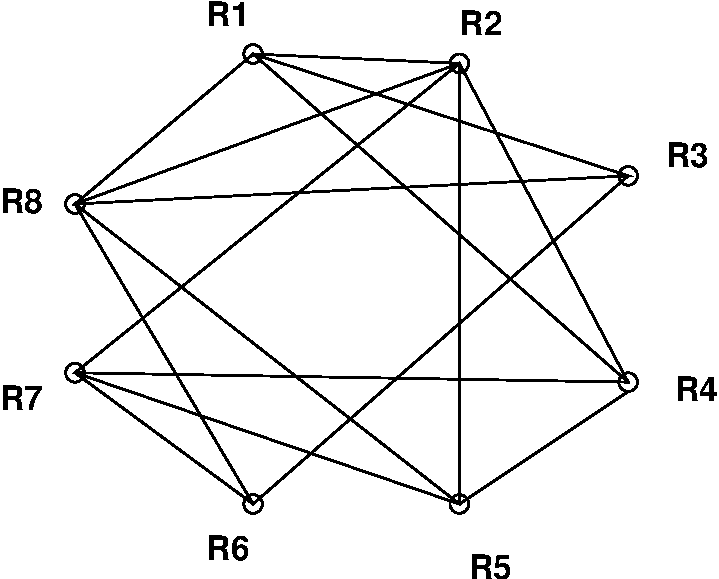
\includegraphics[height=2in]{S09_PS6_schedule.pdf}
\end{center}
}

\ppart{10}
Show a coloring of this graph using the fewest possible
colors.  What schedule of recitations does this imply?

\solution{
Four colors are necessary and sufficient. To see why they
are \emph{sufficient}, consider the coloring:
\begin{center}
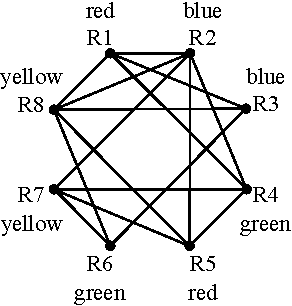
\includegraphics[height=2in]{S09_PS6_schedule_colored.pdf}
\end{center}
This corresponds to the following assignment of recitations to four
time slots:
\begin{enumerate}

\item R1, R5

\item R2, R3

\item R4, R6

\item R7, R8

\end{enumerate}
Other schedules are also possible.

To see why 4 colors are \emph{necessary}, look at the subgraph defined
by the vertices for R2, R4, R5, and R7.  This is the complete graph on 4
vertices, and it obviously needs 4 colors.
}

\eparts

\end{problem}

% Problem
\begin{problem}{20}
Suppose you have a graph as shown below. Every node on the left is adjacent 
to every node on the right except the node directly across from it.
\begin{center}
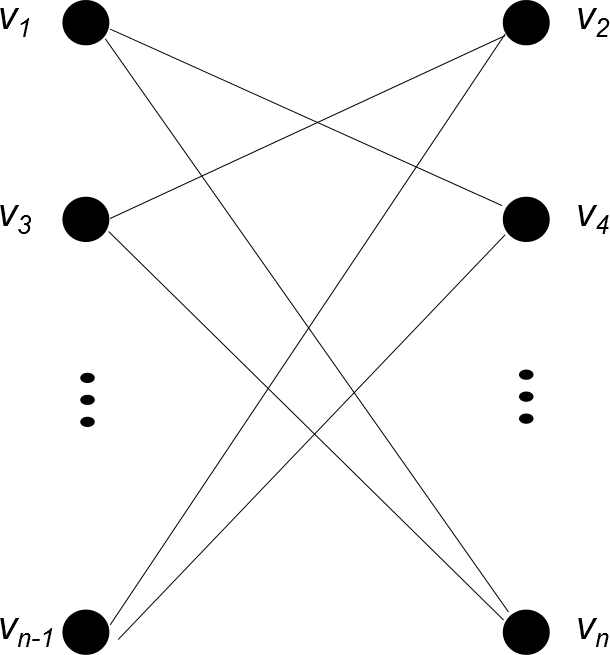
\includegraphics[height = 2in]{coloring}
\end{center}

\bparts

% part a
\ppart{5}
Find the chromatic number of the graph.

% part a solution
\solution{
We can color each node on the left side with red and each node on the right 
with blue since no edges form between nodes on the same side. Thus, the 
chromatic number is 2.
}

% part b
\ppart{5}
The graph pictured above is often referred to as \textit{bipartite}.

\begin{definition*}
A graph $G = (V,E)$ is \underline{bipartite} if the set of vertices, $V$, can 
be split into two subsets $V_l$ and $V_r$ such that all edges in $G$ connect 
nodes in $V_l$ to nodes in $V_r$. 
\end{definition*}

Now recall from lecture the Greedy Coloring Algorithm: \\
\textbf{Greedy Coloring Algorithm:} For a graph $G = (V,E)$ and an ordering 
of vertices $v_1, v_2, \cdots, v_n$
\begin{enumerate}
\item Color $v_1$ with a new color $c_1$.
\item For each vertex $v_i$, if $v_i$ shares an edge with with any earlier vertex,
    $v_j$, colored $c_k$, then it cannot be colored $c_k$. Choose the lowest available
    color for $v_i$.
\end{enumerate}

Find an ordering of the vertices $\{v_1, v_2, \cdots, v_n\}$ such that the 
Greedy Coloring Algorithm uses exactly 2 colors.
% part b solution
\solution{
Since none of the vertices on the left share an edge, we can color all of 
them with the same color, so we iterate through all the left nodes, then all 
the right nodes with the ordering, $v_1, v_3, v_5, \cdots v_{n-1}, \cdots, v_2, v_4, \cdots, v_n$. 
The left side uses only one color and the right side uses only one color 
similar to the solution in part (a).
}

% part c
\ppart{5}
Find an ordering such that the Greedy Coloring Algorithm uses exactly $n/2$ colors.
% part c solution
\solution{
Notice that alternating across left and right with the greedy algorithm forces us to pick a new color 
every time we are on the left side. Thus, we can choose the ordering $v_1, v_2, \cdots 
v_{n/2}, \cdots v_n$ to get $n/2$ colors.
}

% part d
\ppart{5}
Prove your answer in part (c) by induction for all even integers $n$.
% part d solution
\solution{
\begin{proof}
$P(n)$ is defined to be: For a bipartite graph with $n$ vertices (labeled in 
the pattern as shown in the graph), with edges as shown in the graph, 
applying the Greedy Coloring Algorithm to the vertex ordering $v_1, v_2 \cdots
 v_n$ uses exactly $n/2$ colors for all even integers $n$. In addition, the coloring consists of the first $n/2$ colors on each side across from one another.

{ \bf Base Case } (n = 2) There are no edges in this case, so the Greedy 
Coloring Algorithm uses only one color.

{ \bf Inductive Step }
Assume that $P(n)$ is true. We will 
show that this implies $P(n+2)$. Denote our two new nodes $v_{n+1}$ and $v_{n+2
}$. $v_{n+1}$ is connected to $\{v_2, v_4, \cdots v_n\}$ and $v_{n+2}$ is 
connected to $\{v_1, v_3,  \cdots v_{n-1} \}$. Since by $P(n)$, $v_{n+1}$ is 
connected to $n/2$ different colors, the Greedy Coloring Algorithm will 
choose a different color $c_{n/2 + 1}$. For $v_{n+2}$,  the Greedy Algorithm 
will color it $c_{n/2 + 1}$ since its connected to $v_1, v_3, \cdots v_{n-1}$ 
which are the first $n/2$ colors. Thus, the new nodes are a both a new color.\\

Thus, by induction, $P(n+2)$ is true.

\end{proof}
}
\eparts

\end{problem}

\begin{problem}{15}
For each of the following pairs of graphs, either define an isomorphism
between them, or prove that there is none.  (We write $ab$ as shorthand
for the edge from $a$ to $b$).

\bparts

\ppart{5}
\begin{align*}
G_1\text{ with }& V_1 = \set{1,2,3,4,5,6},\ E_1= \set{12,23,34,14,15,35,45}\\
G_2\text{ with }& V_2 = \set{1,2,3,4,5,6},\ E_2= \set{12,23,34,45,51,24,25}
\end{align*}

\solution{Not isomorphic: $G_2$ has a node, 2, of degree 4, but the maximum degree
in $G_1$ is 3.}

\ppart{5}
\begin{align*}
G_3\text{ with } &V_3 = \set{1,2,3,4,5,6},\ E_3= \set{12,23,34,14,45,56,26}\\
G_4\text{ with } &V_4 = \set{a,b,c,d,e,f},\ E_4= \set{ab,bc,cd,de,ae,ef,cf}
\end{align*}

\solution{
Isomorphic (two isomorphisms) with the vertex correspondences: \\
$1f, 2c, 3d, 4e, 5a, 6b$ \\
or $1f, 2e, 3d, 4c, 5b, 6a$
}

\ppart{5}
\begin{align*}
G_5\text{ with } & V_5 = \set{a,b,c,d,e,f,g,h},\ E_5= \set{ab,bc,cd,ad,ef,fg,gh,he,dh,bf}\\
G_6\text{ with } & V_6 = \set{s,t,u,v,w,x,y,z},\ E_6=\set{st,tu,uv,sv,wx,xy,yz,wz,sw,vz}
\end{align*}

\solution{
Not isomorphic: they have the same number of vertices, edges, and set of
vertex degrees.  But the degree 2 vertices of $G_1$ are all adjacent to
two degree 3 vertices, while the degree 2 vertices of $G_2$ are all
adjacent to one degree 2 vertex and one degree 3 vertex.
}

\eparts

\end{problem}

\begin{problem}{15}
Let $G = (V,E)$ be a graph. A {\em matching} in $G$ is a set $M \subset E$ such that no two edges in $M$ are incident on a common vertex.

Let $M_1$, $M_2$ be two matchings of $G$. Consider the new graph $G' = (V, M_1 \cup M_2)$ (i.e. on the same vertex set, whose edges consist of all the edges that appear in either $M_1$ or $M_2$). Show that $G'$ is bipartite.

{\em Helpful definition}: A {\em connected component} is a subgraph of a graph consisting of
some vertex and every node and edge that is connected to that vertex.

\solution{
\begin{proof}

Proof by induction on the number of vertices $n$:

\textbf{Induction hypothesis:}
$P(n)$ is defined to be:  Let $G$ be a graph with $n$ vertices and matchings $M_1$ and $M_2$. Let $G' = (V, M_1 \cup M_2)$. Then $G'$ is bipartite.

\textbf{Base case:} $G$ has only one vertex and so is bipartite. 
$P(1)$ holds.

\textbf{Inductive step:} We will assume $P(n)$ in order to prove $P(n+1)$.

Let $G$ be a graph with $n+1$ vertices.  We will remove a vertex $v$ from $G$ to obtain an $n$ vertex graph, $G_1$, with vertex set $V_1$. If we remove $v$ we will be in one of the following cases:


\textbf{Case 1:} $v$ is in none of the edges in $M_1$ nor $M_2$.

By our inductive hypothesis we know that since $G_1$ has $n$ vertices and $M_1$ and $M_2$ are matchings of $G_1$, then $G_1'=(V_1, M_1 \cup M_2)$ is bipartite. Since $G_1'$ is bipartite, there exists a partition of the vertices into two sets, $L$ and $R$ such that every edge is incident to a vertex in $L$ and to a vertex in $R$. We can now add $v$ to either set and obtain a bipartite representation of $G'$.

\textbf{Case 2:} $v$ is in an edge in either $M_1$ or $M_2$, we will assume, without loss of generality, that $v$ is in an edge in $M_1$.

Suppose the edge $v-x$ is in $M_1$, now remove $v-x$ from $M_1$ to obtain $M_1'$.

Now by our inductive hypothesis we know that since $G_1$ has $n$ vertices and $M_1'$ and $M_2$ are matchings of $G_1$, then $G_1'=(V_1, M_1' \cup M_2)$ is bipartite. Since $G_1'$ is bipartite, there exists a partition of the vertices into two sets, $L$ and $R$ such that every edge is incident to a vertex in $L$ and to a vertex in $R$. 

We know that the vertex $x$ is in either $L$ or $R$. We can just add vertex $v$ to the other set, along with edge $v-x$, and we obtain a valid partitioning of $L$ and $R$ for our graph $G'$. 



\textbf{Case 3:} $v$ is in both $M_1$ and $M_2$

Suppose the edge $v-x$ is in $M_1$ and $v-y$ is in $M_2$, now remove  those edges from $M_1$ and $M_2$ to obtain $M_1'$ and $M_2'$.

Now by our inductive hypothesis we know that since $G_1$ has $n$ vertices and $M_1'$ and $M_2'$ are matchings of $G_1$, then $G_1'=(V_1, M_1' \cup M_2')$ is bipartite. Since $G_1'$ is bipartite, there exists a partition of the vertices into two sets, $L$ and $R$ such that every edge is incident to a vertex in $L$ and to a vertex in $R$. 

If $x$ and $y$ in the same set, either $L$ or $R$, then we can just add $v$ to the other set, and add edges $v-x$ and $v-y$ to obtain $G'$. So our graph remains bipartite. 

If $x$ and $y$ are on different sides of $L$ and $R$, then either $x$ and $y$ are in the same connected component or they are in different connected components. If $x$ and $y$ are in different connected components, then each connected component has a corresponding set of $L$ and $R$ vertices, such that there are edges only within that component. Let's say that the first component has left and right vertices in the set $L_1$ and $R_1$, and the second component has sets $L_2$ and $R_2$, where $L=L_1 \cup L_2$ and $R=R_1 \cup R_2$. Now if we swap $L_1$ and $R_1$ -- that is we define $L=R_1 \cup L_2$ and $R=L_1 \cup R_2$ -- then our graph will remain bipartite, as there were edges only within the connected components. But after the swapping $x$ and $y$ will be in the same set, $L$ or $R$, and as before we can just add $v$ to the other set to get a bipartite graph for $G'$ as desired. 

Now we will show that it is impossible for $x$ and $y$ to be on opposite sides and in the same component. 

Suppose for a contradiction that $x$ and $y$ are in the same connected component and $x$ and $y$ are both in $L$. Then since they are in the same connected component there is a path from $x$ to $y$ say $x-v_1, v_1-v_2, \ldots, v_k-y$, where $k$ is even. Then the edges $x-v_1$ and $v_2-v_3$, $v_4-v_5, \ldots, v_k-y$ must all be in the same matching (otherwise we will have two edges incident on the same vertex in the
same matching). This is a contradiction since our original $M_1$ cannot have any edge with $x$ and $M_2$ cannot have any edge with $y$ (since a matching has only one edge incident to a vertex). So this cannot be the case and $x$ and $y$ must be on the same side.

Hence we conclude that in all cases $G'$ is bipartite.

Therefore by induction our claim holds.
\end{proof}

}
\end{problem}

\end{document}
